\setcounter{figure}{0}

\section{29th October 2023: I AM the way, the truth and the life}
\subsection*{Text: John 14:1-6}
  \begin{quote}
    [1] “Let not your hearts be troubled. Believe in God; believe also in me. [2] In my Father’s house are many rooms. If it were not so, would I have told you that I go to prepare a place for you? [3] And if I go and prepare a place for you, I will come again and will take you to myself, that where I am you may be also. [4] And you know the way to where I am going.” [5] Thomas said to him, “Lord, we do not know where you are going. How can we know the way?” [6] Jesus said to him, “I am the way, and the truth, and the life. No one comes to the Father except through me.
  \end{quote}
\subsection*{Notes}
\begin{itemize}
  \item{There’s a psychological phenomenon called “choice paralysis”, which is when there are too many choices, we cant make a choice. There are an infinite array of lifestyle choices today. There are many different value systems in our world today. For example, which religious tradition (or none) to choose to identify with. This is especially true today, in our increasingly polarised and pluralistic world.}
  \item{For example, the issue of “right and wrong”. In the past, society largely could collectively decide whether something is right or wrong (not that society is always correct). But right now there are so many choices. }
  \item{Apart from society, there is also an objective moral standard which also tells us what “right and wrong” are. The fact that an objective moral standard exists is plain from the fact that we all have moral intuitions that are quite universally agreed upon, such as the disgust at the thought of decapitating babies for fun. But we still have a choice whether we want to believe in this objective moral standard or not, and we still have a choice whether we want to believe that God is the source of this objective moral standard.}
  \item{Apart from our moral intuitions, in each of us, there is a longing for God. As CS Lewis said, “if there is a longing in our souls that the things of the world cannot fulfil, then i must be made for another world”. Our hearts are restless until they find their rest in God. This longing comes from God, and it is because we are made by God and we are made by God. But due to our sin, there is now a chasm between God and us. But the good news is that Jesus came to bridge this chasm.}
  \item{In our text today, it is said that Jesus is the Way, the Truth and the Life. In all of these three words, we see that Jesus is the path back to God, to what we were made for.}
  \item{With respect to Jesus being the Way, we see that Jesus gives us the direction back to God. Since we all have a longing for the rest that only comes from God, we seek to fulfil that longing through many ways. But all those other ways lead to futility. On the other hand, Jesus is the Way out of all our futility in life, out of all our sins, and also Jesus is the Way to the Father. And Jesus being the Way is different from the claims of the other religion. Christianity is not a set of rules. Jesus being the Way does not mean that Jesus gives us a set of rules to obey in an impersonal manner. Jesus being the Way means that He helps us and walks with us to the Father, and helps us to obey the Father.}
  \item{In our world today, there are a lot of fake news, especially online. E.g, the information (or disinformation) war online due to the israel-hamas conflict. Falsehood is so dangerous, and the greatest falsehood is by the grestest scammer, the devil. The devil peddles falsehoods to us every day, such as “there are no way out”, “you are worthless”. The purpose of these falsehoods is to lead us away from God. Jesus being the truth means that we can trust in Jesus, and that when we trust Jesus, our foundation is secure. }
  \item{Finally, we know that as we are, because of sin, we are spiritually dead. We are spiritually dead because we are alienated from God. Sin is a transgression against God, it is when we set ourselves as the king of our own life instead of God. The wages of sin is death, and the wages are paid to us in this life and especially in the life to come. Because of our sin, we experience the consequences of sin in this life. E.g, self-destructive lifestyles like alcoholism and pornography. We also experience the consequences of sin in the next life, which is eternal separation from God. But the gift of God is eternal life through Jesus Christ our Lord.}
  \item{Jesus being the life means that He brings us back to the Father, and hence we can experience eternal life. This eternal life is eternal fellowship with God in the life to come, spending our life in God’s presence, in whom only our life has meaning. And this eternal life is also for this life, when we have fellowship with God and our life is renewed; instead of finding meaning in worthless things, our life has a new identity and also our life has a new direction.}
  % \item{\begin{figure}[H]
  %   \centering
  %   % 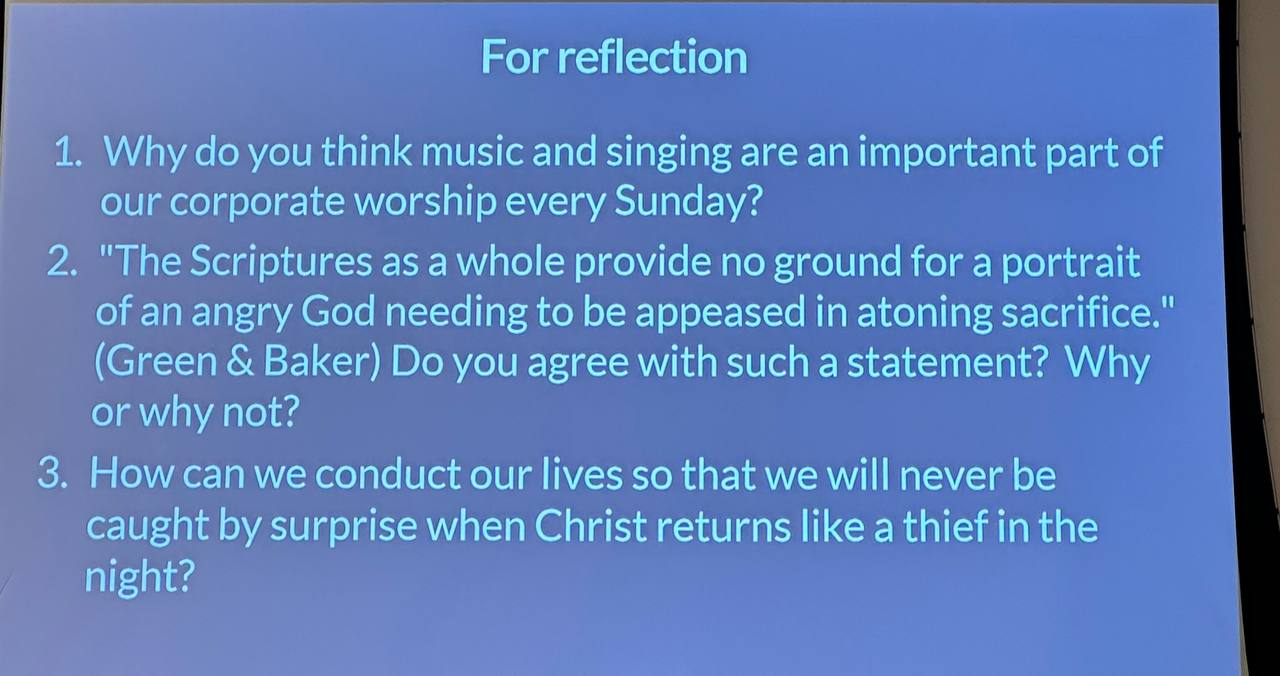
\includegraphics[width=0.8\textwidth, trim={0cm 0cm 0cm 0cm},clip]{Figures/marchSermon4Reflections.jpg}
  %   \includegraphics[width=0.8\textwidth, trim={0cm 0cm 0cm 0cm},clip]{example-image-a}
  %   \caption[]{Reflection questions for this sermon}
  %   \label{}
  % \end{figure}}
\end{itemize}